\acao{Ação 3.2.2.1 – Implantação dos modelos de gestão}

\phantomsection
\addcontentsline{toc}{subsection}{1. Contextualização}
\subsection*{1. Contextualização}

A ação estrutura os modelos de gestão responsáveis pela operação e pela manutenção dos sistemas de abastecimento de água e das soluções de esgotamento sanitário implantados na atividade. Os objetivos são: definir, com as prefeituras e as comunidades, o arranjo de gestão de cada sistema; constituir ou regularizar as associações de saneamento rural; instituir a tarifa; e estruturar três unidades regionais de apoio técnico às entidades gestoras (IAT, 2026a; IAT, 2026b).

O Paraná não dispõe de política estadual de saneamento rural que estabeleça modelo de gestão para esses serviços. As iniciativas existentes são descentralizadas, concentram-se no abastecimento de água e são executadas pela Sanepar, por serviços municipais, por arranjos entre o Estado e os municípios e, em parte dos casos, pelas próprias comunidades (IAT, 2026a).

A autogestão comunitária, predominante no meio rural, apresenta deficiências de capacidade técnica, financeira e institucional e carece de apoio do poder público, o que compromete a regularidade e a qualidade da prestação. A dispersão das comunidades e a limitação de pessoal e de recursos dos municípios agravam esse quadro (BRASIL, 2019; IAT, 2026a).

A ação responde pela sustentabilidade dos investimentos da atividade. Sem entidade gestora habilitada a operar o sistema, cobrar a tarifa e executar a manutenção, os poços, as redes e as soluções de esgotamento sanitário tendem à deterioração em poucos anos; por esse motivo, o modelo de gestão é pactuado antes das obras e acompanha cada sistema até a entrega. A contribuição da ação é medida pelo indicador de associações de saneamento rural com modelo de gestão adotado.

\textbf{Inclui:} a definição e o enquadramento jurídico do modelo; a pactuação com os municípios, formalizada em Termo de Cooperação; a constituição ou a regularização das associações e a adesão das famílias; a elaboração de estatutos, manuais e cartilhas; a instituição da tarifa, com tarifa social; a estruturação das três unidades regionais de apoio (equipe técnica, sede, veículo, geração de energia fotovoltaica e custeio de operação e manutenção); e o acompanhamento das entidades gestoras até o encerramento.

\textbf{Não inclui:} as obras dos sistemas de abastecimento de água e das soluções de esgotamento sanitário, o trabalho técnico-social com as famílias e a formulação da política estadual de saneamento rural, objeto de atividade própria do subcomponente.

\textbf{Valor previsto:} R\$~6,90 milhões (empréstimo BIRD: R\$~6,90 milhões; contrapartida: R\$~0,00 milhões), conforme a planilha PSH\_CUSTO\_Consolidada.

\phantomsection
\addcontentsline{toc}{subsection}{2. Área de atuação}
\subsection*{2. Área de atuação}

A ação abrange as comunidades atendidas pelos sistemas coletivos de abastecimento de água do IAT, selecionadas pelos seguintes critérios: 70 ou mais domicílios ocupados; município classificado como de médio baixo ou de médio desempenho no Índice Ipardes de Desempenho Municipal (IPDM); e prioridade para demandas já encaminhadas ao IAT e para associações que já operam sistemas. A seleção preliminar indicou 83 comunidades, com 5.810 domicílios, sendo o número mínimo de domicílios o requisito de viabilidade da gestão (IAT, 2026a). Os modelos de gestão aplicam-se também às associações constituídas no Programa Sanepar Rural.

A Figura~\ref{mapa} apresenta o mapa inicial das áreas potenciais de atuação: 2.571 aglomerados de domicílios rurais situados a menos de 350 m entre si, classificados em nove faixas de número de domicílios, com os limites das associações de municípios e os 112 municípios consorciados ao Consórcio Intermunicipal de Saneamento do Paraná (CISPAR). A presença do consórcio indica as regiões com base institucional para o arranjo intermunicipal, e as maiores concentrações de domicílios (Região Metropolitana de Curitiba, Centro-Sul e Sudeste do Estado) indicam as localizações candidatas às unidades regionais de apoio. A localização das três unidades é definida após a seleção final das comunidades.

\begin{figure}[H]
  \centering
  \caption{Áreas prioritárias, associações de municípios, CISPAR e concentração de domicílios rurais}\label{mapa}
  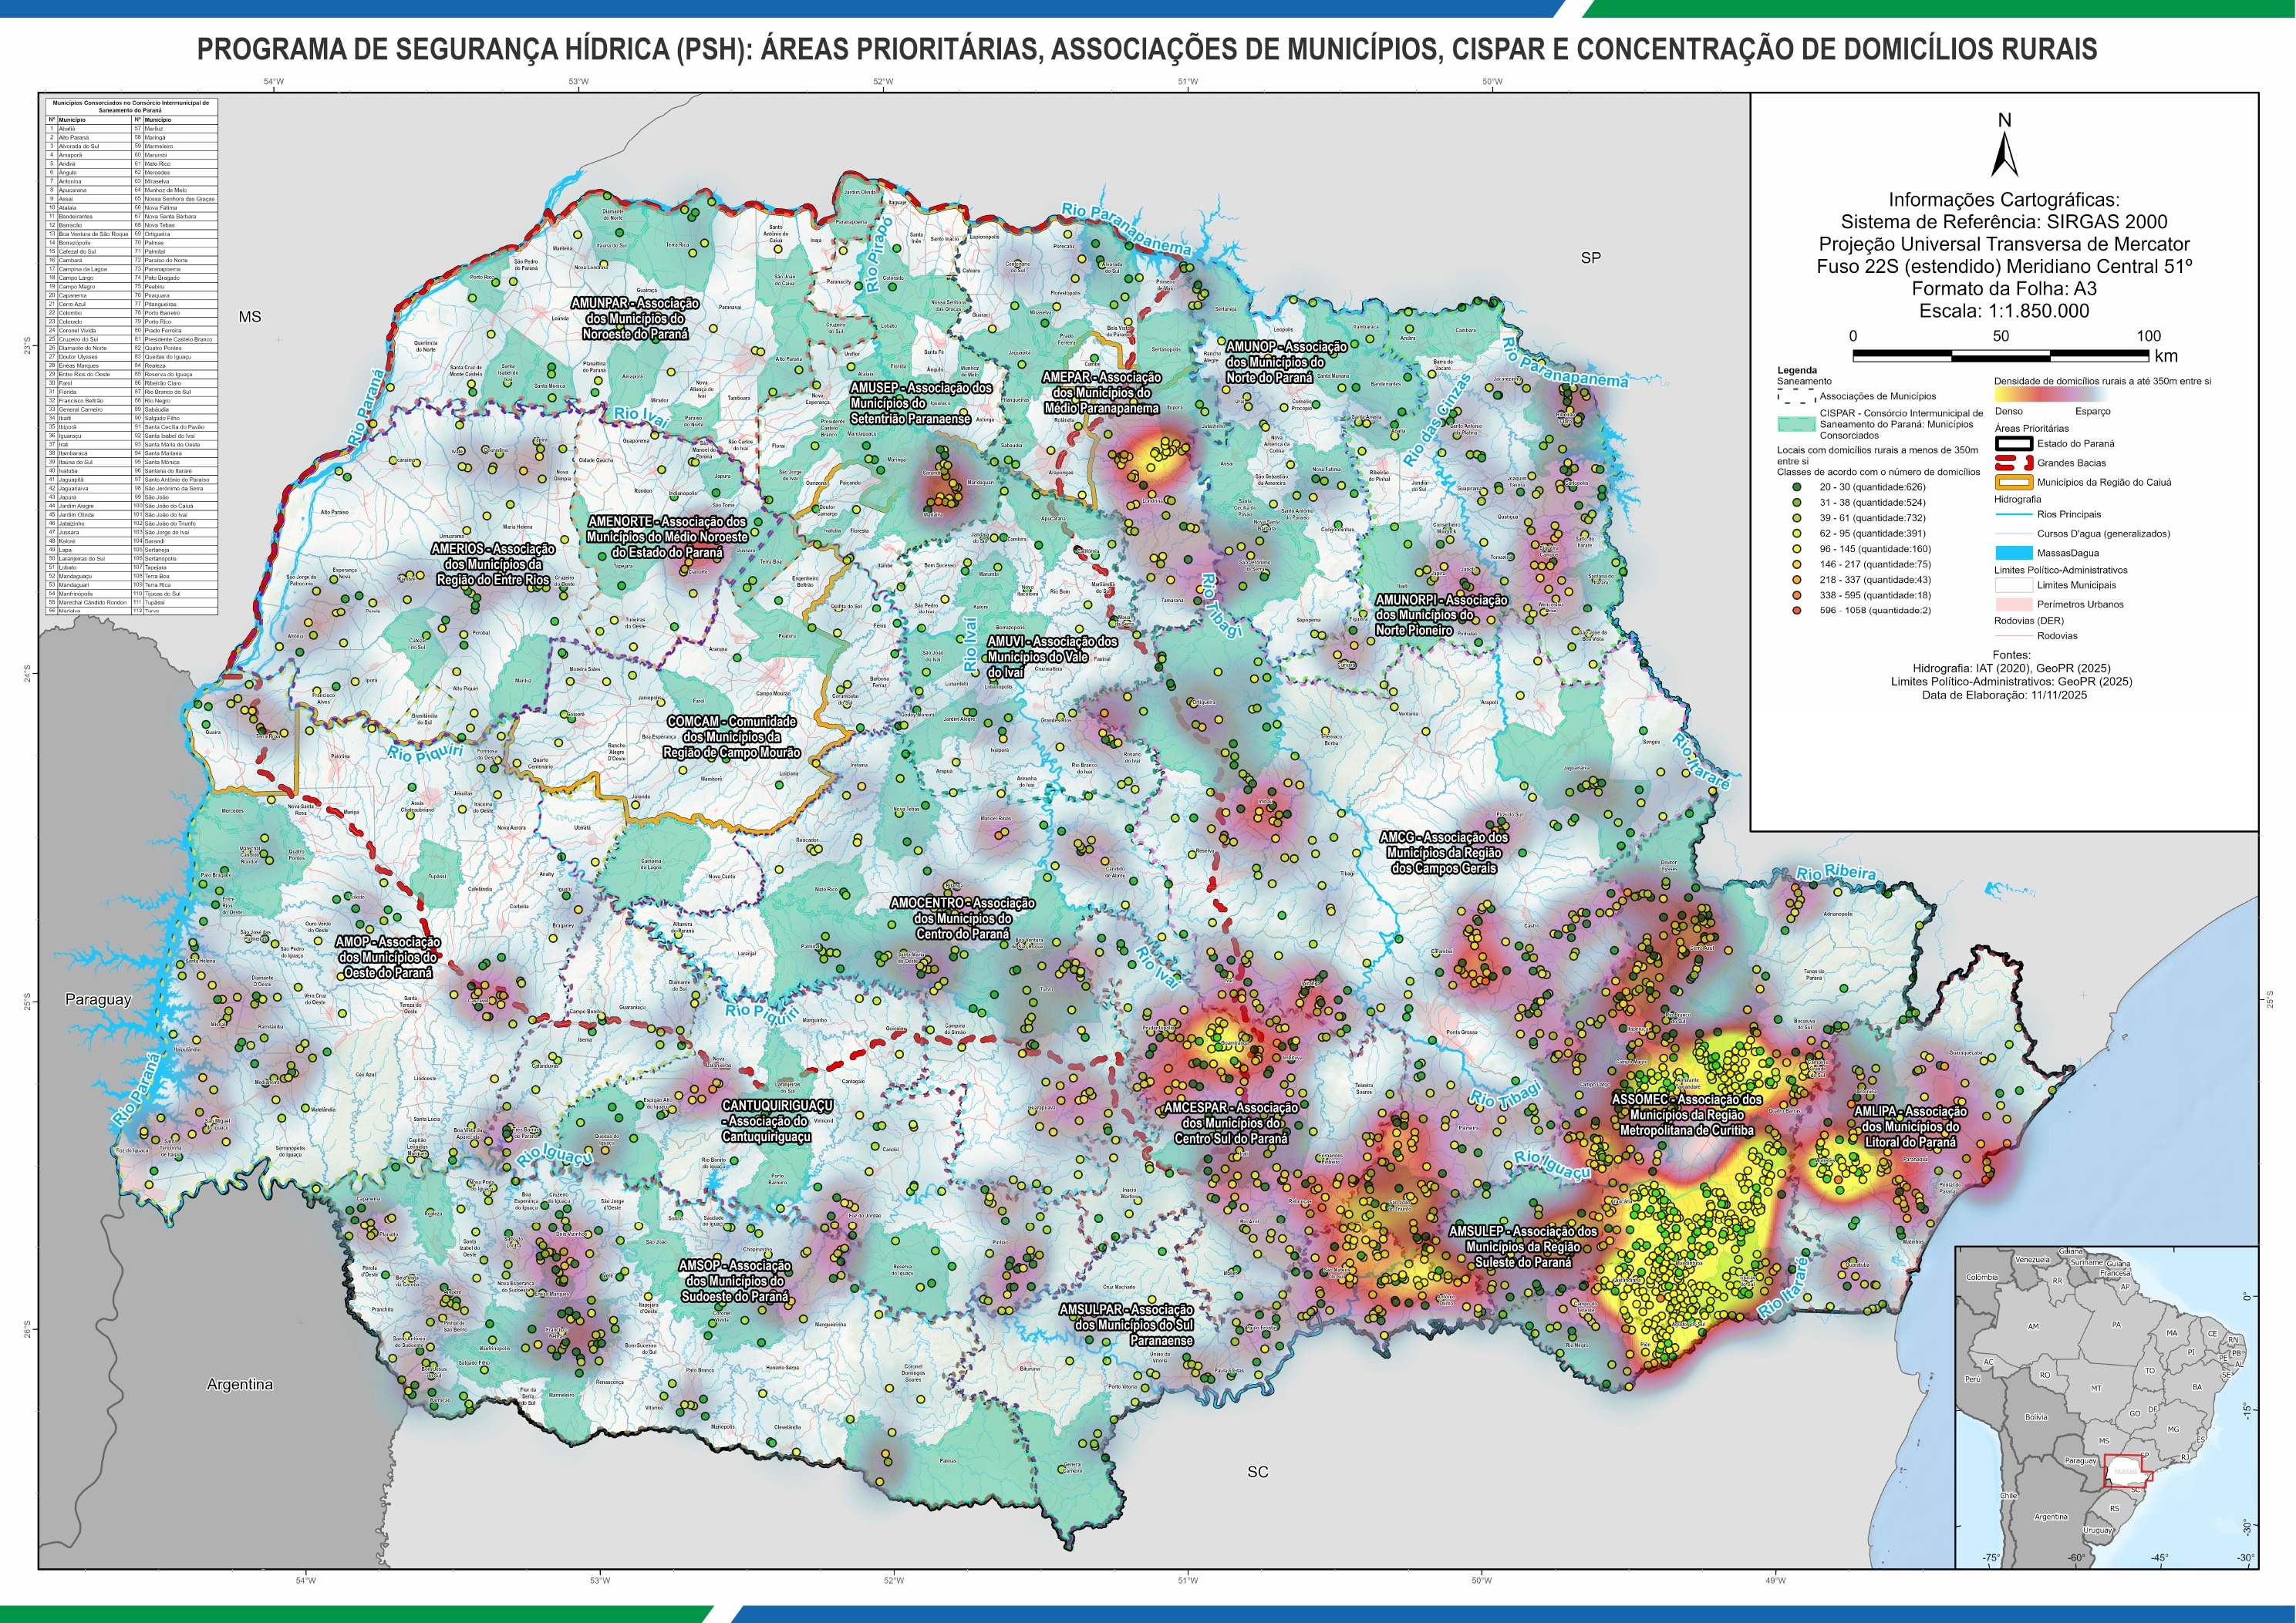
\includegraphics[width=16.00cm]{figuras/f-mapa.jpg}
  \fonteMOP{Fonte: IAT e IDR-Paraná (2025). Hidrografia: IAT (2020) e GeoPR (2025); limites político-administrativos: GeoPR (2025).}
  % Texto alternativo: Mapa do Paraná com as áreas prioritárias do PSH-PR, as associações de municípios, os municípios do CISPAR e os aglomerados de domicílios rurais.
\end{figure}

\pendencia{O Acordo de Empréstimo, item (j)(vii) das definições, exige a identificação das áreas rurais da Parte 3.2 no MOP. O mapa representa o potencial de atuação, e não as 83 comunidades selecionadas; incluir a lista ou o mapa das comunidades e a localização das três unidades regionais.}

\pendencia{Os logos institucionais foram removidos do mapa, conforme o Guia de Identidade Visual (seção 2.6). Na versão final, refazer o mapa sobre a base cartográfica oficial (IAT/ITCG), com as áreas do Programa na cor do Caderno C3 e 40\% de transparência (seção 5.4).}

\phantomsection
\addcontentsline{toc}{subsection}{3. Arranjo institucional e partes interessadas}
\subsection*{3. Arranjo institucional e partes interessadas}

A ação é coordenada pelo IAT, por meio da Diretoria de Saneamento Ambiental e Recursos Hídricos (DISAR), responsável pela definição do modelo, pela pactuação com os municípios e pela constituição e pelo acompanhamento das entidades gestoras. A Secretaria de Estado das Cidades (SECID) valida o modelo de gestão e a tarifa. A UGP acompanha a execução e consolida o reporte ao Banco Mundial.

\pendencia{Indicar a gerência do IAT responsável pela ação (instituição, diretoria e gerência).}

As partes interessadas são:

\begin{itemize}
  \item \textbf{Coexecutores:} a Secretaria de Estado da Agricultura e do Abastecimento (SEAB), na mobilização social e na articulação local, e a Sanepar, nas associações constituídas no Programa Sanepar Rural;
  \item \textbf{Intervenientes:} a SECID, que valida o modelo e a tarifa; as prefeituras, que participam da governança, celebram o Termo de Cooperação, aprovam a lei autorizativa, quando exigida, e apoiam as associações; os consórcios públicos intermunicipais, como o CISPAR, na hipótese de arranjo consorciado; e as empresas contratadas para a equipe técnica e a estrutura das unidades regionais;
  \item \textbf{Comunidades e associações de moradores:} participam da definição do modelo, constituem a entidade gestora e operam os sistemas.
\end{itemize}

Os beneficiários diretos são as associações de saneamento rural e as famílias das comunidades atendidas, que passam a dispor de operação regular, tarifa instituída e suporte técnico. Os beneficiários indiretos são os municípios, que passam a contar com arranjo de gestão para o saneamento rural, e a população das bacias, beneficiada pela manutenção adequada dos sistemas.

\phantomsection
\addcontentsline{toc}{subsection}{4. Processo de execução operacional}
\subsection*{4. Processo de execução operacional}

A ação compreende seis etapas, da definição do modelo ao encerramento dos Termos de Cooperação (Figura~\ref{raias-3221}). Duas premissas orientam a sequência: o modelo de gestão é pactuado antes do início das obras, e nenhum sistema é entregue sem entidade gestora constituída e capacitada para operá-lo.

\begin{figure}[H]
  \centering
  \caption{Fluxograma da implantação dos modelos de gestão: entradas, etapas por responsável e saídas}\label{raias-3221}
  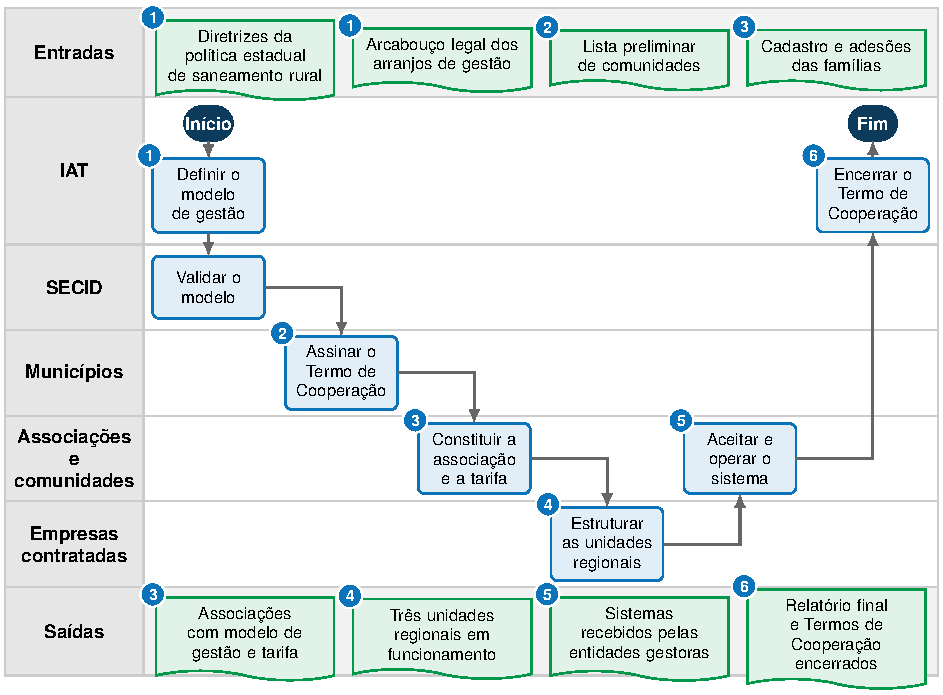
\includegraphics[width=15.96cm]{figuras/g-raias-3221.pdf}
  \fonteMOP{Fonte: IAT (2026).}
  % Texto alternativo: Fluxograma em raias da implantação dos modelos de gestão, com uma raia por instituição, as etapas numeradas na raia do executor, as entradas no topo e as saídas na base.
\end{figure}

\phantomsection
\subsubsection*{4.1 Etapa 1: Estudos preliminares e definição do modelo}

\textbf{Atividades:} seleção dos instrumentos de gestão; definição dos parceiros, dos critérios e dos indicadores; enquadramento jurídico da proposta; e definição da estratégia de comunicação do modelo. Estão em análise três alternativas de arranjo (Quadro~\ref{alternativas}).

Na primeira alternativa, a associação de moradores opera o sistema da respectiva localidade. Na condição de organização da sociedade civil, a associação submete-se ao Marco Regulatório das Organizações da Sociedade Civil (MROSC), e o uso da infraestrutura pública é formalizado por Acordo de Cooperação, após a aprovação de lei municipal autorizativa (BRASIL, 2014).

Na segunda, as associações filiam-se a uma central que lhes presta apoio técnico, administrativo e financeiro. Trata-se do modelo do Sistema Integrado de Saneamento Rural (SISAR) do Ceará, que, em agosto de 2025, atendia mais de 1,13 milhão de pessoas, cerca de 56\% da população rural do estado, em 174 municípios e 1.466 localidades (CEARÁ, 2025). As Centrais de Associações Comunitárias da Bahia adotam arranjo equivalente e executaram 16.888 novas ligações de água e a recuperação de outras 5.297, em 49 municípios (BAHIA, 2022).

\begin{quadro}[H]
  \caption{Alternativas de modelo de gestão e respectivo amparo legal}\label{alternativas}
  \footnotesize\renewcommand{\arraystretch}{1.25}\setlength{\tabcolsep}{5pt}
  \begin{tabular}{>{\raggedright\arraybackslash}p{\dimexpr 0.1874\linewidth-2\tabcolsep\relax}>{\raggedright\arraybackslash}p{\dimexpr 0.2709\linewidth-2\tabcolsep\relax}>{\raggedright\arraybackslash}p{\dimexpr 0.2709\linewidth-2\tabcolsep\relax}>{\raggedright\arraybackslash}p{\dimexpr 0.2709\linewidth-2\tabcolsep\relax}}
    \rowcolor{azulEscuro}\textcolor{white}{\textbf{Aspecto}} & \textcolor{white}{\textbf{Associação de moradores}} & \textcolor{white}{\textbf{Central de associações}} & \textcolor{white}{\textbf{Consórcio público}} \\
    \textbf{Funcionamento} & Moradores organizados operam o sistema da localidade, com apoio da prefeitura & Associações filiadas a uma central, que presta apoio técnico, administrativo e financeiro & Municípios consorciados prestam o serviço de forma associada \\ \arrayrulecolor{cinza20}\hline
    \rowcolor{cinza5}\textbf{Amparo legal} & MROSC (Lei nº~13.019/2014) & MROSC; a nota técnica cita também o Decreto nº~11.599/2023 e a Portaria nº~2.777/2025 da Fundação Nacional de Saúde (Funasa) & Lei dos Consórcios Públicos (Lei nº~11.107/2005) e Lei nº~11.445/2007 \\ \arrayrulecolor{cinza20}\hline
    \textbf{Instrumento} & Acordo de Cooperação, após lei municipal que autoriza a cessão dos ativos & Acordo de Cooperação com o poder público, após lei municipal autorizativa & Alteração do contrato de consórcio; contrato de rateio; cessão de uso dos ativos \\ \arrayrulecolor{cinza20}\hline
    \rowcolor{cinza5}\textbf{Referência} & Associações de moradores que já operam sistemas no Paraná & SISAR (CE): 1,13 milhão de pessoas em 1.466 localidades; Centrais de Associações (BA) & CISPAR: 112 municípios consorciados no Paraná \\ \noalign{\global\arrayrulewidth=1pt}\arrayrulecolor{azulEscuro}\hline\noalign{\global\arrayrulewidth=0.4pt}
  \end{tabular}
  \fonteMOP{Fonte: IAT (2026), com base em IAT (2026a), CEARÁ (2025) e BAHIA (2022).}
  \notaMOP{Nota: em todas as alternativas, o modelo é definido com a prefeitura e a comunidade, mediante abordagem participativa, com tarifa social e capacitação dos operadores.}
\end{quadro}

Na terceira, os municípios prestam o serviço de forma associada, por meio de consórcio público (BRASIL, 2005). Esta é a alternativa preliminarmente indicada para o Paraná, em razão da participação de grande parte dos municípios em consórcios, a exemplo dos 112 municípios consorciados ao CISPAR. O objeto do consórcio existente pode ser ampliado para o abastecimento de água e o esgotamento sanitário rurais, mediante alteração contratual aprovada em assembleia e ratificada por lei de cada ente.

O contrato de rateio define a contribuição anual de cada município, e os poços, as redes e os reservatórios podem ser cedidos ao consórcio, com reversão ao município ao término do contrato. O arranjo proporciona ganho de escala, compartilha a estrutura técnica e administrativa e confere continuidade à gestão entre mandatos. A nota técnica do componente cita, ainda, o Decreto nº~11.599/2023 e a Portaria Funasa nº~2.777/2025 como fundamento dos arranjos associativos no marco legal do saneamento atualizado pela Lei nº~14.026/2020 (IAT, 2026a).

\pendencia{Conferir o fundamento legal citado pela nota técnica. O Decreto nº~11.599/2023 trata da prestação regionalizada e do apoio técnico e financeiro da União; a Portaria Funasa nº~2.777/2025 consta no portal da Funasa como seleção de propostas de abastecimento de água, esgotamento sanitário e melhorias sanitárias domiciliares em áreas rurais, e não como diretriz de modelo de gestão. Ver a planilha de referências normativas.}

\pendencia{A nota técnica prevê contrato de programa no arranjo consorciado. A Lei nº~14.026/2020 alterou a Lei nº~11.445/2007 e restringiu esse instrumento na prestação de serviços de saneamento; confirmar com a assessoria jurídica o instrumento adequado à prestação pelo consórcio.}

\textbf{Entradas:} diretrizes da política estadual de saneamento rural, quando disponíveis; experiências de referência; legislação aplicável.

\textbf{Responsáveis:} IAT (executa), com consulta à SEAB e às prefeituras; SECID (valida o modelo).

\textbf{Produto:} modelo de gestão definido, com enquadramento jurídico.

\pendencia{O modelo de gestão encontra-se em definição. Registrar neste item a alternativa adotada e o parecer jurídico, após a aprovação.}

\phantomsection
\subsubsection*{4.2 Etapa 2: Pactuação com municípios e comunidades}

\textbf{Atividades:} a pactuação inicia-se pelo município e estende-se à comunidade (Figura~\ref{adesao}). O IAT define os critérios, seleciona as comunidades e sensibiliza as prefeituras; o município formaliza a adesão e celebra com o IAT o Termo de Cooperação, que estabelece as obrigações das partes até a entrega dos sistemas. Quando o arranjo envolve cessão de bens públicos, o município aprova a lei autorizativa; em seguida, o IAT contata a comunidade, que manifesta o interesse por meio de contrato de pré-adesão.

\begin{figure}[H]
  \centering
  \caption{Seleção e adesão dos municípios e das comunidades, por responsável}\label{adesao}
  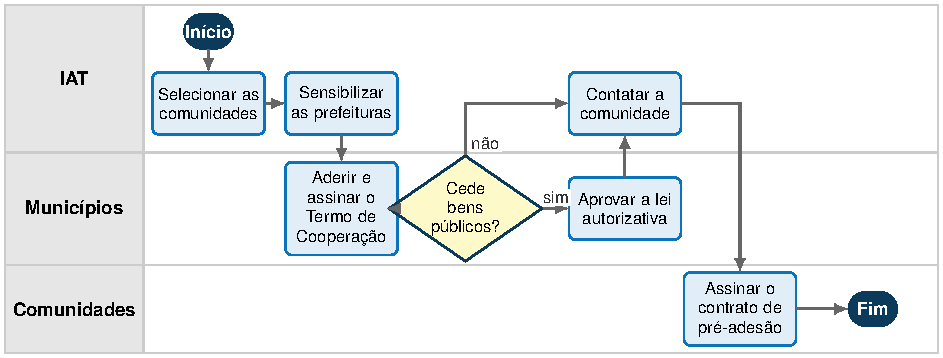
\includegraphics[width=15.96cm]{figuras/f-adesao.pdf}
  \fonteMOP{Fonte: IAT (2026), com base em IAT (2026b).}
  % Texto alternativo: Fluxograma em raias do IAT, dos municípios e das comunidades, da seleção das comunidades à pré-adesão, com a decisão sobre a lei autorizativa.
\end{figure}

\textbf{Entradas:} modelo de gestão definido (Etapa 1); lista preliminar de comunidades; minuta do Termo de Cooperação.

\textbf{Responsáveis:} IAT e prefeituras (executam); SEAB e comunidades (consultadas); IAT (aprova os termos).

\textbf{Produto:} Termos de Cooperação assinados e contratos de pré-adesão.

\phantomsection
\subsubsection*{4.3 Etapa 3: Constituição das entidades gestoras}

\textbf{Atividades:} após a adesão da comunidade, o IAT apoia a constituição ou a regularização da associação de saneamento rural: elabora o estatuto, os manuais e as cartilhas, formaliza a adesão de cada família e acompanha o registro da associação. A tarifa é aprovada em assembleia, com tarifa social para as famílias de baixa renda, e validada pela SECID. A etapa utiliza o cadastro e os termos de adesão do trabalho técnico-social e é concluída antes do início da obra de cada sistema.

\textbf{Entradas:} contratos de pré-adesão; cadastro e termos de adesão das famílias (trabalho técnico-social).

\textbf{Responsáveis:} IAT e associações (executam); prefeituras (consultadas); SECID (valida a tarifa).

\textbf{Produto:} associação regularizada, com tarifa instituída.

\phantomsection
\subsubsection*{4.4 Etapa 4: Estruturação das unidades regionais de apoio}

\textbf{Atividades:} cada uma das três unidades previstas na planilha de custos constitui estrutura regional de apoio às associações, com equipe técnica, sede, veículo, geração de energia fotovoltaica e custeio de operação e manutenção (IAT, 2026a). As unidades elaboram os manuais de desempenho operacional, estruturam o monitoramento e capacitam os dirigentes e os operadores das associações. Implanta-se uma unidade por ano, de 2028 a 2030, conforme a entrada em operação dos primeiros sistemas.

\textbf{Entradas:} modelo e localização das unidades definidos; associações constituídas.

\textbf{Responsáveis:} IAT (executa e aprova) e empresas contratadas (executam); associações (informadas).

\textbf{Produto:} unidade regional em funcionamento e pessoal capacitado.

\pendencia{A nota técnica do componente estima as três unidades em R\$~6,63 milhões, e a planilha de custos, em R\$~6,90 milhões; prevalece a planilha. Confirmar a composição de cada unidade e a fonte de custeio da operação após 2030.}

\phantomsection
\subsubsection*{4.5 Etapa 5: Entrega dos sistemas e acompanhamento}

\textbf{Atividades:} concluída a obra, a entrega é formalizada em reunião técnica com a comunidade e a entidade gestora, que atesta o recebimento por termo de aceite. A partir da entrega, a entidade gestora opera e mantém o sistema com suporte da unidade regional, e o IAT avalia o desempenho semestralmente, com base nos dados registrados no Sistema de Gestão Ambiental e de Recursos Hídricos (SIGARH) e na plataforma GeoPR. As entregas acompanham o cronograma de implantação dos sistemas de abastecimento.

\textbf{Entradas:} sistemas de abastecimento de água e soluções de esgotamento sanitário concluídos; associação regularizada.

\textbf{Responsáveis:} IAT e entidade gestora (executam); entidade gestora (aceita o sistema); prefeituras (consultadas).

\textbf{Produto:} termos de aceite assinados e relatórios semestrais de desempenho.

\phantomsection
\subsubsection*{4.6 Etapa 6: Encerramento}

\textbf{Atividades:} consolidação dos resultados, relatório final, prestação de contas e encerramento do Termo de Cooperação com cada município.

\textbf{Entradas:} relatórios semestrais; Termos de Recebimento Definitivo dos sistemas.

\textbf{Responsáveis:} IAT (executa); UGP (valida).

\textbf{Produto:} relatório final e Termos de Cooperação encerrados.

\phantomsection
\subsubsection*{4.7 Modalidade de execução}

O item de custo é a implantação do modelo de gestão: três unidades de R\$~2,3 milhões, no total de R\$~6,90 milhões, com recursos do empréstimo do BIRD. Na planilha, o produto consta como “Sistema coletivo de abastecimento de água e individual de tratamento de efluentes”.

As Etapas 1, 2, 3, 5 e 6 são executadas diretamente pela equipe do IAT, com Termo de Cooperação com cada município. A Etapa 4 é executada mediante licitação, conforme o Caderno AQ: serviços de consultoria para a equipe técnica das unidades, aquisição de bens (veículos e sistemas fotovoltaicos) e serviços de adequação das sedes.

\pendencia{Confirmar no Plano de Aquisições a divisão dos processos da Etapa 4 (consultoria, bens e serviços).}

\pendencia{Completar as remissões aos cadernos transversais com a seção correspondente (por exemplo, “Caderno AQ, seção 4”), conforme o Guia de Identidade Visual (seção 2.5), quando a numeração desses cadernos estiver definida.}

\phantomsection
\addcontentsline{toc}{subsection}{5. Matriz de responsabilidades}
\subsection*{5. Matriz de responsabilidades}

O Quadro~\ref{raci-3221} apresenta o papel de cada parte em cada etapa.

\begin{quadro}[H]
  \caption{Matriz de responsabilidades da implantação dos modelos de gestão}\label{raci-3221}
  \footnotesize\renewcommand{\arraystretch}{1.25}\setlength{\tabcolsep}{3pt}
  \begin{tabular}{>{\raggedright\arraybackslash}p{\dimexpr 0.2536\linewidth-2\tabcolsep\relax}>{\centering\arraybackslash}p{\dimexpr 0.0882\linewidth-2\tabcolsep\relax}>{\centering\arraybackslash}p{\dimexpr 0.0882\linewidth-2\tabcolsep\relax}>{\centering\arraybackslash}p{\dimexpr 0.0882\linewidth-2\tabcolsep\relax}>{\centering\arraybackslash}p{\dimexpr 0.0882\linewidth-2\tabcolsep\relax}>{\centering\arraybackslash}p{\dimexpr 0.0882\linewidth-2\tabcolsep\relax}>{\centering\arraybackslash}p{\dimexpr 0.0882\linewidth-2\tabcolsep\relax}>{\centering\arraybackslash}p{\dimexpr 0.2173\linewidth-2\tabcolsep\relax}}
    \rowcolor{azulEscuro}\textcolor{white}{\textbf{Parte}} & \textcolor{white}{\textbf{E1}} & \textcolor{white}{\textbf{E2}} & \textcolor{white}{\textbf{E3}} & \textcolor{white}{\textbf{E4}} & \textcolor{white}{\textbf{E5}} & \textcolor{white}{\textbf{E6}} & \textcolor{white}{\textbf{Produto final}} \\
    IAT & \raci{R} & \raci{R} \raci{A} & \raci{R} & \raci{R} \raci{A} & \raci{R} & \raci{R} & \raci{R} \\ \arrayrulecolor{cinza20}\hline
    \rowcolor{cinza5}SECID & \raci{A} & \raci{I} & \raci{A} & \raci{I} & \raci{I} & \raci{I} & \raci{A} \\ \arrayrulecolor{cinza20}\hline
    SEAB & \raci{C} & \raci{C} & – & – & \raci{I} & \raci{I} & \raci{I} \\ \arrayrulecolor{cinza20}\hline
    \rowcolor{cinza5}Prefeituras & \raci{C} & \raci{R} & \raci{C} & \raci{I} & \raci{C} & \raci{C} & \raci{I} \\ \arrayrulecolor{cinza20}\hline
    Associações e comunidades & – & \raci{C} & \raci{R} & \raci{I} & \raci{A} & \raci{I} & \raci{R} \\ \arrayrulecolor{cinza20}\hline
    \rowcolor{cinza5}Empresas contratadas & – & – & – & \raci{R} & – & – & – \\ \arrayrulecolor{cinza20}\hline
    UGP & \raci{I} & \raci{I} & \raci{I} & \raci{I} & \raci{I} & \raci{A} & \raci{I} \\ \noalign{\global\arrayrulewidth=1pt}\arrayrulecolor{azulEscuro}\hline\noalign{\global\arrayrulewidth=0.4pt}
  \end{tabular}
  \fonteMOP{Fonte: IAT (2026).}
  \notaMOP{Nota: E1 a E6 correspondem às Etapas 1 a 6 do item 4. \raci{R} executa (pode haver mais de um); \raci{A} aprova ou valida o produto (um por etapa); \raci{C} é consultado previamente; \raci{I} é informado posteriormente. Produto final: associações de saneamento rural com modelo de gestão adotado.}
\end{quadro}

\phantomsection
\addcontentsline{toc}{subsection}{6. Metas, indicadores e comprovação}
\subsection*{6. Metas, indicadores e comprovação}

A meta física da ação é a implantação de três unidades regionais de apoio, uma por ano, de 2028 a 2030 (Quadro~\ref{metas-3221}). As entidades gestoras são constituídas à medida que os sistemas são concluídos.

\begin{quadro}[H]
  \caption{Metas anuais da implantação dos modelos de gestão}\label{metas-3221}
  \footnotesize\renewcommand{\arraystretch}{1.25}\setlength{\tabcolsep}{3pt}
  \begin{tabular}{>{\raggedright\arraybackslash}p{\dimexpr 0.2095\linewidth-2\tabcolsep\relax}>{\raggedright\arraybackslash}p{\dimexpr 0.1268\linewidth-2\tabcolsep\relax}>{\raggedleft\arraybackslash}p{\dimexpr 0.0794\linewidth-2\tabcolsep\relax}>{\raggedleft\arraybackslash}p{\dimexpr 0.0794\linewidth-2\tabcolsep\relax}>{\raggedleft\arraybackslash}p{\dimexpr 0.0794\linewidth-2\tabcolsep\relax}>{\raggedleft\arraybackslash}p{\dimexpr 0.0794\linewidth-2\tabcolsep\relax}>{\raggedleft\arraybackslash}p{\dimexpr 0.0794\linewidth-2\tabcolsep\relax}>{\raggedleft\arraybackslash}p{\dimexpr 0.0794\linewidth-2\tabcolsep\relax}>{\raggedleft\arraybackslash}p{\dimexpr 0.0794\linewidth-2\tabcolsep\relax}>{\raggedleft\arraybackslash}p{\dimexpr 0.1081\linewidth-2\tabcolsep\relax}}
    \rowcolor{azulEscuro}\textcolor{white}{\textbf{Produto}} & \textcolor{white}{\textbf{Unidade}} & \centering\arraybackslash \textcolor{white}{\textbf{Ano 1}} & \centering\arraybackslash \textcolor{white}{\textbf{Ano 2}} & \centering\arraybackslash \textcolor{white}{\textbf{Ano 3}} & \centering\arraybackslash \textcolor{white}{\textbf{Ano 4}} & \centering\arraybackslash \textcolor{white}{\textbf{Ano 5}} & \centering\arraybackslash \textcolor{white}{\textbf{Ano 6}} & \centering\arraybackslash \textcolor{white}{\textbf{Ano 7}} & \centering\arraybackslash \textcolor{white}{\textbf{Total}} \\
    Unidades regionais do modelo de gestão implantadas & unidades & – & 1 & 1 & 1 & – & – & – & 3 \\ \noalign{\global\arrayrulewidth=1pt}\arrayrulecolor{azulEscuro}\hline\noalign{\global\arrayrulewidth=0.4pt}
  \end{tabular}
  \fonteMOP{Fonte: Planilha PSH\_CUSTO\_Consolidada, versão v2408 (PARANÁ, 2026).}
  \notaMOP{Nota: Ano 1 = 2027 e Ano 7 = 2033. Na planilha, o produto consta como “Sistema coletivo de abastecimento de água e individual de tratamento de efluentes”.}
\end{quadro}

O Quadro~\ref{ind-3221} reúne os indicadores de andamento e de resultado da ação. O principal é o indicador de associações de saneamento rural com modelo de gestão adotado, medido pelo número acumulado de associações que formalizaram a adoção do modelo.

\begin{quadro}[H]
  \caption{Indicadores da implantação dos modelos de gestão}\label{ind-3221}
  \footnotesize\renewcommand{\arraystretch}{1.25}\setlength{\tabcolsep}{3pt}
  \begin{tabular}{>{\raggedright\arraybackslash}p{\dimexpr 0.3165\linewidth-2\tabcolsep\relax}>{\raggedright\arraybackslash}p{\dimexpr 0.1378\linewidth-2\tabcolsep\relax}>{\raggedleft\arraybackslash}p{\dimexpr 0.1102\linewidth-2\tabcolsep\relax}>{\raggedleft\arraybackslash}p{\dimexpr 0.1599\linewidth-2\tabcolsep\relax}>{\raggedright\arraybackslash}p{\dimexpr 0.2756\linewidth-2\tabcolsep\relax}}
    \rowcolor{azulEscuro}\textcolor{white}{\textbf{Indicador}} & \textcolor{white}{\textbf{Unidade}} & \centering\arraybackslash \textcolor{white}{\textbf{Linha de base (2025)}} & \centering\arraybackslash \textcolor{white}{\textbf{Meta}} & \textcolor{white}{\textbf{Frequência e fonte dos dados}} \\
    Associações de saneamento rural com modelo de gestão adotado (indicador do componente) & associações (acumulado) & 0 & 122 & Anual; IAT, Sanepar e cadastro das associações \\ \arrayrulecolor{cinza20}\hline
    \rowcolor{cinza5}Unidades regionais de apoio em funcionamento & unidades & 0 & 3 & Anual; IAT \\ \arrayrulecolor{cinza20}\hline
    Sistemas recebidos pela entidade gestora com termo de aceite & sistemas & 0 & 83 & Semestral; IAT \\ \arrayrulecolor{cinza20}\hline
    \rowcolor{cinza5}Domicílios atendidos com tarifa instituída & domicílios & 0 & 5.810 & Anual; associações e IAT \\ \noalign{\global\arrayrulewidth=1pt}\arrayrulecolor{azulEscuro}\hline\noalign{\global\arrayrulewidth=0.4pt}
  \end{tabular}
  \fonteMOP{Fonte: IAT (2026).}
\end{quadro}

\pendencia{O MOP de março previa 122 associações até 2032, no período de 2027 a 2032. Atualizar as metas anuais para o período de 2027 a 2033 e explicitar a composição do total (comunidades atendidas pelo IAT e associações do Programa Sanepar Rural).}

Os critérios de aceite e as evidências de comprovação de cada produto constam do Quadro~\ref{aceite-3221}. A sustentabilidade do resultado é verificada após a entrega: a entidade gestora deve estar em operação, com tarifa cobrada, associação ativa e relatório semestral de desempenho.

\begin{quadro}[H]
  \caption{Critérios de aceite e evidências da implantação dos modelos de gestão}\label{aceite-3221}
  \footnotesize\renewcommand{\arraystretch}{1.25}\setlength{\tabcolsep}{5pt}
  \begin{tabular}{>{\raggedright\arraybackslash}p{\dimexpr 0.2150\linewidth-2\tabcolsep\relax}>{\raggedright\arraybackslash}p{\dimexpr 0.3386\linewidth-2\tabcolsep\relax}>{\raggedright\arraybackslash}p{\dimexpr 0.2921\linewidth-2\tabcolsep\relax}>{\raggedright\arraybackslash}p{\dimexpr 0.1543\linewidth-2\tabcolsep\relax}}
    \rowcolor{azulEscuro}\textcolor{white}{\textbf{Produto}} & \textcolor{white}{\textbf{Critério de aceite}} & \textcolor{white}{\textbf{Evidência de comprovação}} & \textcolor{white}{\textbf{Responsável pela validação}} \\
    Modelo de gestão definido & Arranjo definido para cada conjunto de comunidades, com enquadramento jurídico & Nota técnica do modelo e parecer jurídico & SECID \\ \arrayrulecolor{cinza20}\hline
    \rowcolor{cinza5}Termo de Cooperação & Assinado pelo município, com obrigações, prazos e contrapartidas & Termo assinado e publicado & IAT \\ \arrayrulecolor{cinza20}\hline
    Contratos de pré-adesão & Assinados pelas famílias interessadas da comunidade & Contratos assinados; número de associados & IAT \\ \arrayrulecolor{cinza20}\hline
    \rowcolor{cinza5}Associação regularizada & Estatuto registrado e inscrição ativa no Cadastro Nacional da Pessoa Jurídica (CNPJ) & Registro em cartório; comprovante de inscrição no CNPJ & IAT \\ \arrayrulecolor{cinza20}\hline
    Tarifa instituída & Aprovada em assembleia, com tarifa social para famílias de baixa renda & Ata da assembleia; regulamento tarifário & SECID \\ \arrayrulecolor{cinza20}\hline
    \rowcolor{cinza5}Unidade regional em funcionamento & Equipe contratada, sede e veículo em operação & Contratos; termo de recebimento dos bens; relatório de atividades & IAT \\ \arrayrulecolor{cinza20}\hline
    Pessoal capacitado & Conteúdo e carga horária do plano de capacitação cumpridos & Listas de presença e certificados & IAT \\ \arrayrulecolor{cinza20}\hline
    \rowcolor{cinza5}Sistema aceito pela entidade gestora & Sistema recebido sem pendências & Termo de aceite assinado & IAT \\ \arrayrulecolor{cinza20}\hline
    Desempenho acompanhado & Relatório semestral entregue e aprovado & Relatório com dados registrados no SIGARH e no GeoPR & UGP \\ \noalign{\global\arrayrulewidth=1pt}\arrayrulecolor{azulEscuro}\hline\noalign{\global\arrayrulewidth=0.4pt}
  \end{tabular}
  \fonteMOP{Fonte: IAT (2026).}
\end{quadro}

\phantomsection
\addcontentsline{toc}{subsection}{7. Gestão de riscos e impactos ambientais e sociais}
\subsection*{7. Gestão de riscos e impactos ambientais e sociais}

A ação tem natureza institucional e social, e as intervenções físicas restringem-se à adequação das sedes das unidades regionais, de pequeno porte. Os riscos concentram-se na exclusão de famílias vulneráveis ou de comunidades tradicionais, nos conflitos pelo uso da água e na sustentabilidade financeira das associações. O Quadro~\ref{nas-3221} indica as NAS aplicáveis e as respectivas medidas.

As NAS 3, 5, 6 e 8 não se aplicam de forma específica à ação, e a NAS 9 não se aplica ao Programa. Os instrumentos de gestão ambiental e social (Marco de Gestão Ambiental e Social – MGAS, Plano de Engajamento das Partes Interessadas – PEPI e Mecanismo de Queixas e Reclamações – MQR) constam do Caderno AS.

\begin{quadro}[H]
  \caption{Aplicação das Normas Ambientais e Sociais à implantação dos modelos de gestão}\label{nas-3221}
  \footnotesize\renewcommand{\arraystretch}{1.25}\setlength{\tabcolsep}{5pt}
  \begin{tabular}{>{\raggedright\arraybackslash}p{\dimexpr 0.1874\linewidth-2\tabcolsep\relax}>{\raggedright\arraybackslash}p{\dimexpr 0.3716\linewidth-2\tabcolsep\relax}>{\raggedright\arraybackslash}p{\dimexpr 0.4410\linewidth-2\tabcolsep\relax}}
    \rowcolor{azulEscuro}\textcolor{white}{\textbf{NAS}} & \textcolor{white}{\textbf{Aplicação à ação}} & \textcolor{white}{\textbf{Medidas e instrumentos}} \\
    NAS 1 – Avaliação e gestão de riscos & Riscos sociais do modelo: exclusão de famílias, conflitos pelo uso da água e inadimplência & Triagem socioambiental das comunidades; tarifa social; avaliação semestral de desempenho (MGAS) \\ \arrayrulecolor{cinza20}\hline
    \rowcolor{cinza5}NAS 2 – Condições de trabalho & Trabalhadores das empresas que compõem as equipes das unidades regionais & Cláusulas trabalhistas nos contratos; Procedimentos de Gestão de Mão de Obra \\ \arrayrulecolor{cinza20}\hline
    NAS 7 – Povos indígenas e comunidades tradicionais & Comunidades tradicionais ou indígenas nas áreas selecionadas & Identificação na seleção; consulta culturalmente adequada; arranjo compatível com a organização da comunidade (MGAS e PEPI) \\ \arrayrulecolor{cinza20}\hline
    \rowcolor{cinza5}NAS 10 – Engajamento das partes interessadas & Participação das prefeituras e das comunidades na definição do modelo e da tarifa & Reuniões com linguagem acessível; consulta às comunidades; divulgação do Mecanismo de Queixas e Reclamações (PEPI e MQR) \\ \noalign{\global\arrayrulewidth=1pt}\arrayrulecolor{azulEscuro}\hline\noalign{\global\arrayrulewidth=0.4pt}
  \end{tabular}
  \fonteMOP{Fonte: IAT (2026), com base nos instrumentos do Caderno AS.}
\end{quadro}

\phantomsection
\addcontentsline{toc}{subsection}{8. Cronograma}
\subsection*{8. Cronograma}

As etapas acompanham a implantação dos sistemas (Figura~\ref{crono-3221}). A definição do modelo ocorre em 2027; a pactuação, de 2027 a 2030; a constituição das entidades gestoras, de 2028 a 2032, sempre antes da obra de cada sistema; e a estruturação das unidades regionais, uma por ano, de 2028 a 2030. As entregas seguem o cronograma de implantação dos sistemas de abastecimento (5 sistemas em 2028, 10 em 2029, 20 em 2030 e em 2031, 18 em 2032 e 10 em 2033), e a ação é encerrada em 2033.

\begin{figure}[H]
  \centering
  \caption{Cronograma das etapas e das entregas da implantação dos modelos de gestão}\label{crono-3221}
  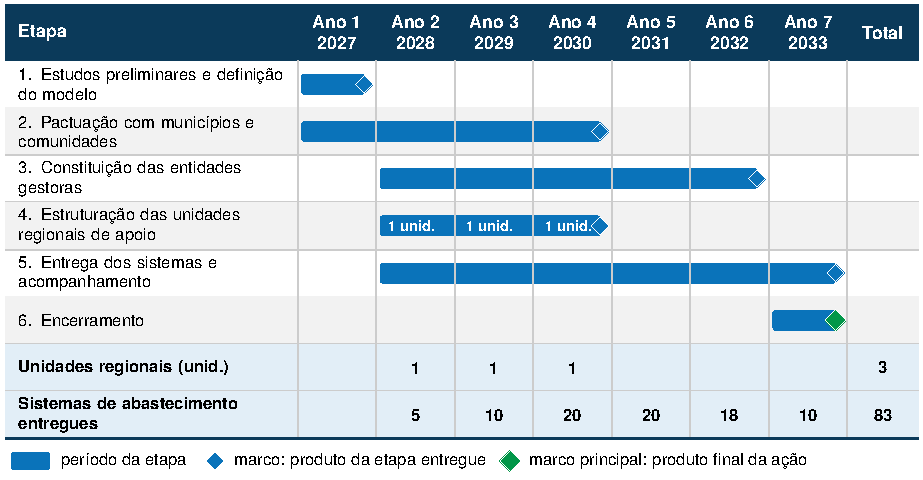
\includegraphics[width=15.64cm]{figuras/g-crono-3221.pdf}
  \fonteMOP{Fonte: IAT (2026), com quantidades da planilha PSH\_CUSTO\_Consolidada (PARANÁ, 2026).}
  % Texto alternativo: Cronograma anual de 2027 a 2033 com as etapas e as quantidades a entregar da implantação dos modelos de gestão.
\end{figure}

\phantomsection
\addcontentsline{toc}{subsection}{9. Interfaces e dependências}
\subsection*{9. Interfaces e dependências}

A ação depende das diretrizes da política estadual de saneamento rural, do cadastro e das adesões do trabalho técnico-social e da conclusão dos sistemas de abastecimento de água e das soluções de esgotamento sanitário. Em contrapartida, fornece às demais ações os municípios aderidos e a entidade gestora definida antes de cada obra, aplica o modelo às associações do Programa Sanepar Rural e alimenta o indicador de associações reportado à UGP (Figura~\ref{interf-3221}).

\begin{figure}[H]
  \centering
  \caption{Interfaces e dependências da implantação dos modelos de gestão}\label{interf-3221}
  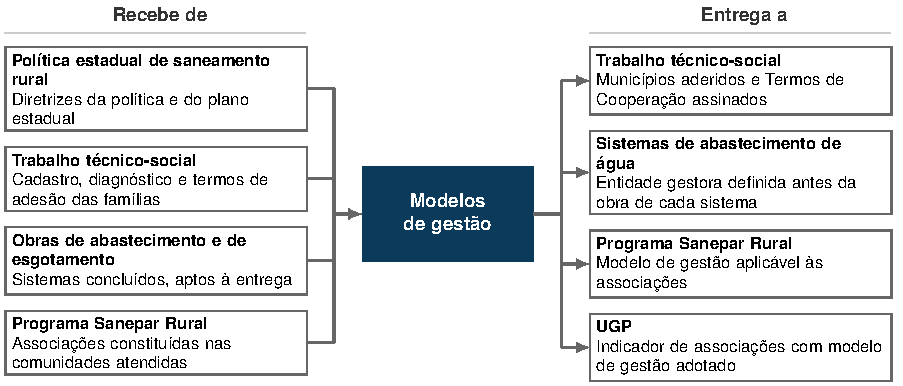
\includegraphics[width=15.30cm]{figuras/g-interf-3221.pdf}
  \fonteMOP{Fonte: IAT (2026).}
  % Texto alternativo: Diagrama das interfaces da implantação dos modelos de gestão: insumos recebidos de outras partes do Programa e produtos entregues a elas.
\end{figure}

\phantomsection
\addcontentsline{toc}{subsection}{10. Documentos complementares}
\subsection*{10. Documentos complementares}

\begin{itemize}
  \item Termo de Cooperação entre o IAT e cada município (minuta a elaborar);
  \item Modelos de estatuto, manuais de desempenho operacional e cartilhas das associações (a elaborar);
  \item Termo de Referência da equipe técnica das unidades regionais (a elaborar);
  \item Lei nº~13.019/2014 (MROSC), Lei nº~11.107/2005 (consórcios públicos), Lei nº~11.445/2007, com a redação da Lei nº~14.026/2020 (marco legal do saneamento), e Decreto nº~11.599/2023;
  \item Programa Nacional de Saneamento Rural (BRASIL, 2019);
  \item Caderno AS (MGAS, PEPI e Mecanismo de Queixas e Reclamações) e Caderno AQ;
  \item Notas técnicas de origem (IAT, 2026a; IAT, 2026b).
\end{itemize}
